\documentclass[10pt]{beamer}\usepackage[]{graphicx}\usepackage[]{color}
%% maxwidth is the original width if it is less than linewidth
%% otherwise use linewidth (to make sure the graphics do not exceed the margin)
\makeatletter
\def\maxwidth{ %
  \ifdim\Gin@nat@width>\linewidth
    \linewidth
  \else
    \Gin@nat@width
  \fi
}
\makeatother

\definecolor{fgcolor}{rgb}{0.345, 0.345, 0.345}
\newcommand{\hlnum}[1]{\textcolor[rgb]{0.686,0.059,0.569}{#1}}%
\newcommand{\hlstr}[1]{\textcolor[rgb]{0.192,0.494,0.8}{#1}}%
\newcommand{\hlcom}[1]{\textcolor[rgb]{0.678,0.584,0.686}{\textit{#1}}}%
\newcommand{\hlopt}[1]{\textcolor[rgb]{0,0,0}{#1}}%
\newcommand{\hlstd}[1]{\textcolor[rgb]{0.345,0.345,0.345}{#1}}%
\newcommand{\hlkwa}[1]{\textcolor[rgb]{0.161,0.373,0.58}{\textbf{#1}}}%
\newcommand{\hlkwb}[1]{\textcolor[rgb]{0.69,0.353,0.396}{#1}}%
\newcommand{\hlkwc}[1]{\textcolor[rgb]{0.333,0.667,0.333}{#1}}%
\newcommand{\hlkwd}[1]{\textcolor[rgb]{0.737,0.353,0.396}{\textbf{#1}}}%
\let\hlipl\hlkwb

\usepackage{framed}
\makeatletter
\newenvironment{kframe}{%
 \def\at@end@of@kframe{}%
 \ifinner\ifhmode%
  \def\at@end@of@kframe{\end{minipage}}%
  \begin{minipage}{\columnwidth}%
 \fi\fi%
 \def\FrameCommand##1{\hskip\@totalleftmargin \hskip-\fboxsep
 \colorbox{shadecolor}{##1}\hskip-\fboxsep
     % There is no \\@totalrightmargin, so:
     \hskip-\linewidth \hskip-\@totalleftmargin \hskip\columnwidth}%
 \MakeFramed {\advance\hsize-\width
   \@totalleftmargin\z@ \linewidth\hsize
   \@setminipage}}%
 {\par\unskip\endMakeFramed%
 \at@end@of@kframe}
\makeatother

\definecolor{shadecolor}{rgb}{.97, .97, .97}
\definecolor{messagecolor}{rgb}{0, 0, 0}
\definecolor{warningcolor}{rgb}{1, 0, 1}
\definecolor{errorcolor}{rgb}{1, 0, 0}
\newenvironment{knitrout}{}{} % an empty environment to be redefined in TeX

\usepackage{alltt}

%% include header:
\usetheme{metropolis}
\usepackage{appendixnumberbeamer}

\usepackage{booktabs}
\usepackage[scale=2]{ccicons}

\usepackage{pgfplots}
\usepgfplotslibrary{dateplot}

\usepackage{xspace}
\newcommand{\themename}{\textbf{\textsc{metropolis}}\xspace}

\usepackage[english]{babel}
\usepackage{dsfont}
\usepackage{amsmath}
\usepackage{amssymb}
\usepackage{amsthm}
\usepackage{amsfonts}


%% Define theme color(s):
%% ---------------------------------------------------------------

\usepackage{xcolor}

\definecolor{metropolis_theme_color}{RGB}{35,55,59}
% \definecolor{metropolis_theme_color}{RGB}{110, 117, 87}

%% Color custimzations:
\definecolor{blue}{RGB}{0,155,164}
\definecolor{lime}{RGB}{175,202,11}
\definecolor{green}{RGB}{0,137,62}
\definecolor{titleblue}{RGB}{112,122,82}
\definecolor{deepskyblue}{RGB}{0,191,255}
\definecolor{mygrey}{RGB}{240,240,240}

% \setbeamercolor{progress bar}{fg=deepskyblue}
% \setbeamercolor{frametitle}{bg=metropolis_theme_color}

%% Shaded for nicer code highlighting:
%% ---------------------------------------------------------------

\usepackage{mdframed}
% \usepackage{verbatim}

% Define Shaded if not defined:
\makeatletter
\@ifundefined{Shaded}{%
  \newenvironment{Shaded}{\begin{snugshade}}{\end{snugshade}}%
}{}
\makeatother

\renewenvironment{Shaded}{
  \begin{mdframed}[
    backgroundcolor=mygrey,
    linecolor=metropolis_theme_color,
    rightline=false,
		leftline=false
  ]}{
  \end{mdframed}
}

%% Title Image:
%% ---------------------------------------------------------------

% Load transparent:
\usepackage{transparent}

% Add titlegraphic:
\titlegraphic{
  \vspace{2cm}
  \hspace{5.03cm}
  \transparent{0.2}
  
\includegraphics[width=8cm]{images/logos/LMU}
}

%% Adjust frame number to be displayd as i/n:
%% ---------------------------------------------------------------
\setbeamertemplate{frame numbering}{%
  \insertframenumber{}/\inserttotalframenumber
}
\makeatother


%% Include latex-math:
%% ---------------------------------------------------------------
% Include latex-math
\DeclareOldFontCommand{\sf}{\normalfont\sffamily}{\mathsf}

\IfFileExists{./latex-math/basic-math.tex}{
  \input{./latex-math/basic-math.tex}
  \input{./latex-math/ml-bagging.tex}
  \input{./latex-math/ml-boosting.tex}
  \input{./latex-math/ml-gp.tex}
  \input{./latex-math/ml-mbo.tex}
  \input{./latex-math/ml-nn.tex}
  \input{./latex-math/ml-svm.tex}
  \input{./latex-math/ml-trees.tex}
}{
  \IfFileExists{./../latex-math/basic-math.tex}{
    \input{./../latex-math/basic-math.tex}
    \input{./../latex-math/basic-ml.tex}
    \input{./../latex-math/ml-bagging.tex}
    \input{./../latex-math/ml-boosting.tex}
    \input{./../latex-math/ml-gp.tex}
    \input{./../latex-math/ml-mbo.tex}
    \input{./../latex-math/ml-nn.tex}
    \input{./../latex-math/ml-svm.tex}
    \input{./../latex-math/ml-trees.tex}
  }{}
}

%% Style URLs
%% ---------------------------------------------------------------

\usepackage{hyperref}

\definecolor{myorange}{RGB}{225, 127, 0}
\renewcommand\UrlFont{\color{myorange}}

%% include template:
%% Footer:
\usepackage{xfrac}
\usepackage{framed, color}

\setbeamertemplate{footline}[text line]{%
    \noindent\hspace*{\dimexpr-\oddsidemargin-1in\relax}%
     \colorbox{metropolis_theme_color}{
     \makebox[\dimexpr\paperwidth-2\fboxsep\relax]{
     \color{mygrey}
     \begin{minipage}{0.33\linewidth}
       \secname
     \end{minipage}\hfill
     \begin{minipage}{0.33\linewidth}
       \centering
       \insertshortauthor
     \end{minipage}\hfill
     \begin{minipage}{0.33\linewidth}
       \flushright
       \insertframenumber{}/\inserttotalframenumber
     \end{minipage}     
     }}%
  \hspace*{-\paperwidth}
}

%% Custom stuff:
\usepackage[]{algorithm2e}
\usepackage{csquotes}
\usepackage{dsfont}
\usepackage{natbib}

%% Title:
%% ----------------------------------------

\title{Compboost}
\subtitle{Modular framework for \textbf{comp}onent-wise \textbf{boost}ing}
\date{10 July 2018}
\author{Daniel Schalk, Janek Thomas, Bernd Bischl \newline daniel.schalk@stat.uni-muenchen.de}
\institute{LMU Munich\\Working Group Computational Statistics}

%% Wrap Shaded around Shunk to have a nices R output:
%% --------------------------------------------------

% Include before begin document to have Schunk:

\let\Oldkframe\kframe
\let\endOldkframe\endkframe

\renewenvironment{kframe}
 {\scriptsize\definecolor{shadecolor}{RGB}{240,240,240}\begin{Shaded}\Oldkframe}
 {\endOldkframe\end{Shaded}\normalsize}

\makeatletter
\let\latexl@section\l@section
\def\l@section#1#2{\begingroup\let\numberline\@gobble\latexl@section{#1}{#2}\endgroup}
\makeatother

\let\oldcite\cite
\renewcommand{\cite}[1]{\beamergotobutton{\oldcite{#1}}}

% \setbeamercolor{button}{bg=metropolis_theme_color,fg=white}
\setbeamercolor{button}{bg=myorange,fg=white}

% \let\oldBeamergotobutton\beamergotobutton
% \renewcommand{\beamergotobutton}[1]{\oldBeamergotobutton{\scriptsize #1}}

\setbeamerfont{bibliography item}{size=\footnotesize}
\setbeamerfont{bibliography entry author}{size=\footnotesize}
\setbeamerfont{bibliography entry title}{size=\footnotesize}
\setbeamerfont{bibliography entry location}{size=\footnotesize}
\setbeamerfont{bibliography entry note}{size=\footnotesize}

\setlength{\parskip}{0pt}

\setlength{\OuterFrameSep}{-4pt}
\makeatletter
\preto{\@verbatim}{\topsep=-10pt \partopsep=-10pt }
\makeatother

%% Content:
%% ----------------------------------------
\IfFileExists{upquote.sty}{\usepackage{upquote}}{}
\begin{document}




\maketitle

\author{Daniel Schalk, Janek Thomas, Bernd Bischl}

% \begin{frame}[plain]{Table of Contents}
% 	\tableofcontents
% \end{frame}

\section{Why Component-Wise Boosting?}
% \addtocounter{framenumber}{-1}


\begin{frame}{Why Component-Wise Boosting?}

\vspace{-0.6cm}

\begin{figure}
  \centering
  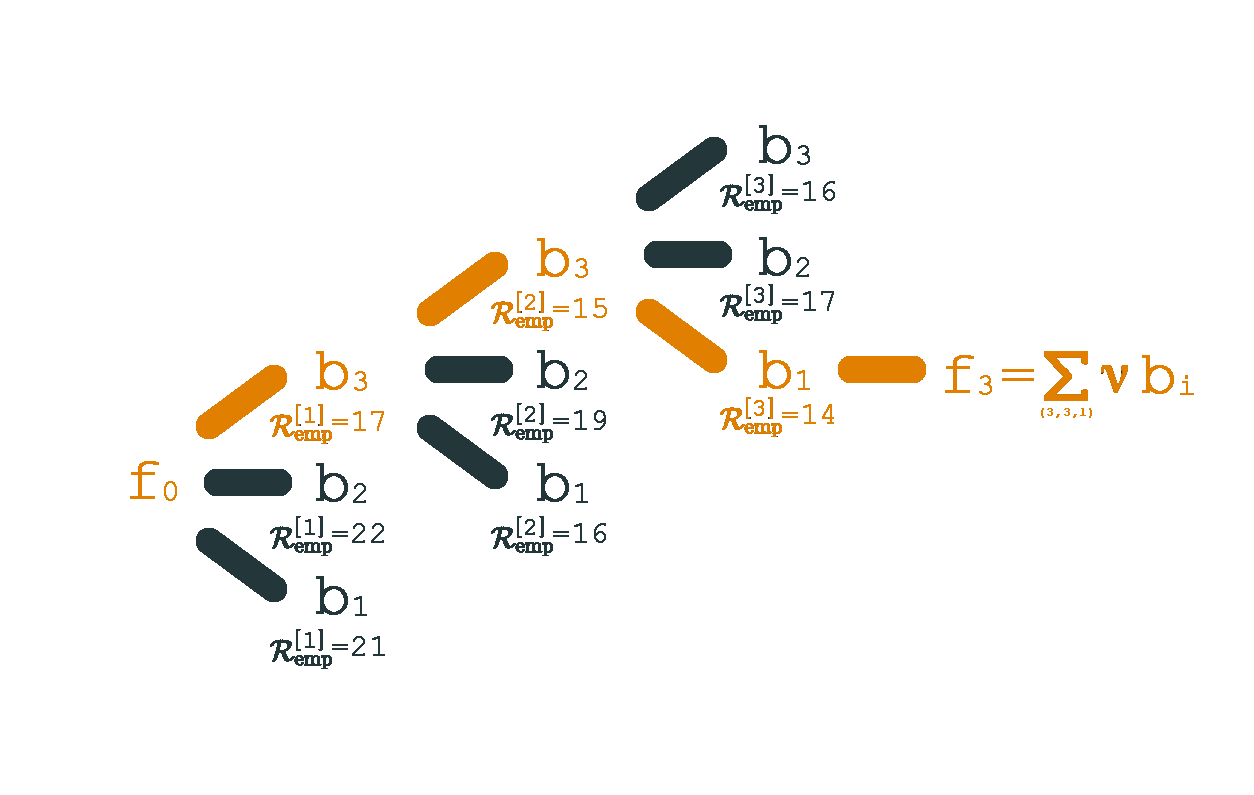
\includegraphics[width=0.75\textwidth]{images/comp_boosting.png}
\end{figure}

\vspace{-1.2cm}
\pause

\begin{itemize}

  \item
    Inherent (unbiased) feature selection  \cite{hofner2011framework}.
    
  \item
    Resulting model is sparse since important effects are selected first and therefore 
    it is able to learn in high-dimensional feature spaces ($p \gg n$).
    
  \item 
    Parameters are updated iteratively. Therefore, the 
    whole trace of how the model evolves is available.    
    
\end{itemize}

\end{frame}



% \begin{frame}[fragile]{Why Component-Wise Boosting?}
% 
% \begin{itemize}
% 
%   \item
%     Inherent (unbiased) feature selection  \cite{hofner2011framework}.
%     
%   \item
%     The resulting model is sparse since important effects are selected first and therefore 
%     it is able to learn in high-dimensional feature spaces ($p \gg n$).
%     
%   \item 
%     The parameters are updated iteratively. Therefore, the 
%     whole trace of how the model evolves is available.    
%     
% \end{itemize}
% 
% \end{frame}



% \begin{frame}{Component-Wise Boosting: The Algorithm}

% \begin{Shaded}
% \begin{algorithm}[H]
% % \KwData{this text}
% \scriptsize
% \KwResult{Component-wise boosting model $\fh(x)$}
% Initialize $\fh^{[0]}(x) = \argmin_{c\in\R} \riske(c)$ \;
%   \For{$m \in \{1, \dots, M\}$}{\vspace{0.2cm}
%     // Update pseudo residuals: \\
%     $r^{[m](i)} = -\left[ \frac{\delta}{\delta f(\xi)} L\left(\yi, f(\xi)\right) \right]_{f = f^{[m-1]}},\ \forall i \in \{1, \dots, n\}$ \;\vspace{0.2cm}
%     // Get index $j^\ast$ of $m$-th base-learner from optimizer:\\
%     \For{$j \in \{1, \dots, J\}$}{
%       // Fit each base-learner $b_j^{[m]}$ to the pseudo residuals: \\
%       $\hat{\theta}_j^{[m]} = \argmin_{\theta_j} \sum\limits_{i=1}^n\left( 
%       \rmi - b_j^{[m]}(\xi, \theta_j)\right)^2$ \;\vspace{0.2cm}
%       // Calculate the SSE of the fitted base-learner:\\
%       $\mathsf{SSE}_j = \sum\limits_{i=1}^n \left(\rmi - b_j^{[m]}(\xi, \hat{\theta}_j)\right)^2$ \; 
%     }
%     // Add selected component to model:\\
%     $\fmh(x) = \fmdh(x) + \beta b^{[m]}_{j^\ast}\left(x, \theta_{j^\ast}^{[m]}\right)$
%   }
% \textbf{Returns:} $\fh(x) = \fmh(x)$\;
% \end{algorithm}
% \end{Shaded}

% \end{frame}


\begin{frame}[fragile]{Available R Packages}

Most popular package for model-based boosting is \texttt{mboost} \parbox{1cm}{\parbox{4cm}{\cite{mboost1}:}}

\begin{itemize}
	
  \item
    Large number of available base-learner and losses.

  \item 
    Extended to more complex problems:
    \begin{itemize}
      \item Functional data \cite{brockhaus2017boosting}
      \item GAMLSS models \cite{mayr2012generalized}
      \item Survival analysis
    \end{itemize}
  \item 
    Extendible with custom base-learner and losses. 

\end{itemize}
\pause

\textbf{So, why another boosting implementation?}

\begin{itemize}

  \item
    Main parts of \texttt{mboost} are written in \texttt{R} and gets slow for large datasets.

  \item 
    Complex implementation:
    \begin{itemize} 
      \item Nested scopes 
      \item Mixture of different \texttt{R} class systems
    \end{itemize}
\end{itemize}

\end{frame}

\section{About Compboost}


\begin{frame}{About compboost}

The \texttt{compboost} package is a fast and flexible framework for model-based boosting completely written in \texttt{C++}:

\begin{itemize}

	\item
	  With \texttt{mboost} as standard, we want to keep the modular principle of defining custom base-learner and losses.

	\item 
	  Completely written in \texttt{C++} and exposed by \texttt{Rcpp} \parbox{0.5cm}{\parbox{3cm}{\cite{Rcpp}}} \cite{eddelbuettel2017exposing} to obtain high performance and full memory control.

	\item
		\texttt{R} API is written in \texttt{R6} to provide convenient wrapper.

	\item 
	  Major parts of the \texttt{compboost} functionality are unit tested against \texttt{mboost} to ensure correctness.

\end{itemize}

\end{frame}


\begin{frame}{Compboost: Functionality}

Main components:

\begin{itemize}

	\item
		Base-learner and loss classes.
	
	\item
		Logger class for early stopping and logging mechanisms.

\end{itemize}

Possible extensions:

\begin{itemize}

	\item
		Custom \texttt{R} or \texttt{C++} base-learner.
	
	\item
		Custom \texttt{R} or \texttt{C++} loss objects.
	
	\item
		Custom logging and stopping rules via custom losses.

\end{itemize}

Custom classes can be defined without recompiling the whole package, even when using \texttt{C++} functions.

\end{frame}

\section{Usecase}


\begin{frame}[fragile]{Initialize Model}

We are interested in modelling the risk of diabetes of female Pima Indians. Interesting features are \texttt{age} and the \texttt{mass}. 

\begin{knitrout}
\definecolor{shadecolor}{rgb}{0.969, 0.969, 0.969}\color{fgcolor}\begin{kframe}
\begin{alltt}
\hlkwd{library}\hlstd{(compboost)}

\hlkwd{data}\hlstd{(PimaIndiansDiabetes,} \hlkwc{package} \hlstd{=} \hlstr{"mlbench"}\hlstd{)}

\hlcom{# Defining a new Compboost object:}
\hlstd{cboost} \hlkwb{=} \hlstd{Compboost}\hlopt{$}\hlkwd{new}\hlstd{(}\hlkwc{data} \hlstd{= PimaIndiansDiabetes,} \hlkwc{target} \hlstd{=} \hlstr{"diabetes"}\hlstd{,}
  \hlkwc{loss} \hlstd{= BinomialLoss}\hlopt{$}\hlkwd{new}\hlstd{())}

\hlcom{# Adding a linear and spline base-learner to the Compboost object:}
\hlstd{cboost}\hlopt{$}\hlkwd{addBaselearner}\hlstd{(}\hlkwc{feature} \hlstd{=} \hlstr{"mass"}\hlstd{,} \hlkwc{id} \hlstd{=} \hlstr{"linear"}\hlstd{, PolynomialBlearner,}
  \hlkwc{degree} \hlstd{=} \hlnum{1}\hlstd{,} \hlkwc{intercept} \hlstd{=} \hlnum{TRUE}\hlstd{)}
\hlstd{cboost}\hlopt{$}\hlkwd{addBaselearner}\hlstd{(}\hlkwc{feature} \hlstd{=} \hlstr{"age"}\hlstd{,} \hlkwc{id} \hlstd{=} \hlstr{"spline"}\hlstd{, PSplineBlearner,}
  \hlkwc{degree} \hlstd{=} \hlnum{3}\hlstd{,} \hlkwc{n.knots} \hlstd{=} \hlnum{10}\hlstd{,} \hlkwc{penalty} \hlstd{=} \hlnum{2}\hlstd{,} \hlkwc{differences} \hlstd{=} \hlnum{2}\hlstd{)}
\end{alltt}
\end{kframe}
\end{knitrout}




\end{frame}

\begin{frame}[fragile]{Initialize Model}

\begin{knitrout}
\definecolor{shadecolor}{rgb}{0.969, 0.969, 0.969}\color{fgcolor}\begin{kframe}
\begin{alltt}
\hlstd{cboost}\hlopt{$}\hlkwd{train}\hlstd{(}\hlnum{2000}\hlstd{,} \hlkwc{trace} \hlstd{=} \hlnum{FALSE}\hlstd{)}
\hlstd{cboost}
\end{alltt}
\begin{verbatim}
## Component-Wise Gradient Boosting
## 
## Trained on PimaIndiansDiabetes with target diabetes
## Number of base-learners: 2
## Learning rate: 0.05
## Iterations: 2000
## Positive class: neg
## Offset: 0.3118
## 
## BinomialLoss Loss:
## 
##   Loss function: L(y,x) = log(1 + exp(-2yf(x))
## 
## 
\end{verbatim}
\end{kframe}
\end{knitrout}


\end{frame}

\begin{frame}[fragile]{Access Results and Continue Training}

\begin{knitrout}
\definecolor{shadecolor}{rgb}{0.969, 0.969, 0.969}\color{fgcolor}\begin{kframe}
\begin{alltt}
\hlstd{cboost}\hlopt{$}\hlkwd{train}\hlstd{(}\hlnum{1000}\hlstd{)} \hlcom{# Set model to iteration 1000}

\hlkwd{table}\hlstd{(cboost}\hlopt{$}\hlkwd{selected}\hlstd{())} \hlcom{# Table of vector of selected base-learner}
\end{alltt}
\begin{verbatim}
## 
##  age_spline mass_linear 
##         611         389
\end{verbatim}
\begin{alltt}
\hlstd{cboost}\hlopt{$}\hlkwd{train}\hlstd{(}\hlnum{3000}\hlstd{)} \hlcom{# Set model to iteration 3000}
\end{alltt}
\begin{verbatim}
## 
## You have already trained 2000 iterations.
## Train 1000 additional iterations.
\end{verbatim}
\begin{alltt}
\hlkwd{str}\hlstd{(cboost}\hlopt{$}\hlkwd{risk}\hlstd{())} \hlcom{# Get vector of inbag risk}
\end{alltt}
\begin{verbatim}
##  num [1:3001] 0.658 0.657 0.655 0.653 0.652 ...
\end{verbatim}
\begin{alltt}
\hlkwd{str}\hlstd{(cboost}\hlopt{$}\hlkwd{coef}\hlstd{())} \hlcom{# Get list of estimated parameter}
\end{alltt}
\begin{verbatim}
## List of 3
##  $ age_spline : num [1:14, 1] 5.581 0.67 1.251 -1.134 0.199 ...
##  $ mass_linear: num [1:2, 1] 3.08 -0.09
##  $ offset     : num 0.312
\end{verbatim}
\end{kframe}
\end{knitrout}

\end{frame}


\begin{frame}[fragile]{Plot Results}

\begin{knitrout}
\definecolor{shadecolor}{rgb}{0.969, 0.969, 0.969}\color{fgcolor}\begin{kframe}
\begin{alltt}
\hlstd{cboost}\hlopt{$}\hlkwd{plot}\hlstd{(}\hlstr{"age_spline"}\hlstd{,} \hlkwc{iters} \hlstd{=} \hlkwd{c}\hlstd{(}\hlnum{100}\hlstd{,} \hlnum{500}\hlstd{,} \hlnum{1000}\hlstd{,} \hlnum{2000}\hlstd{,} \hlnum{3000}\hlstd{))}
\end{alltt}
\end{kframe}
\end{knitrout}

\begin{center}
\begin{knitrout}
\definecolor{shadecolor}{rgb}{0.969, 0.969, 0.969}\color{fgcolor}
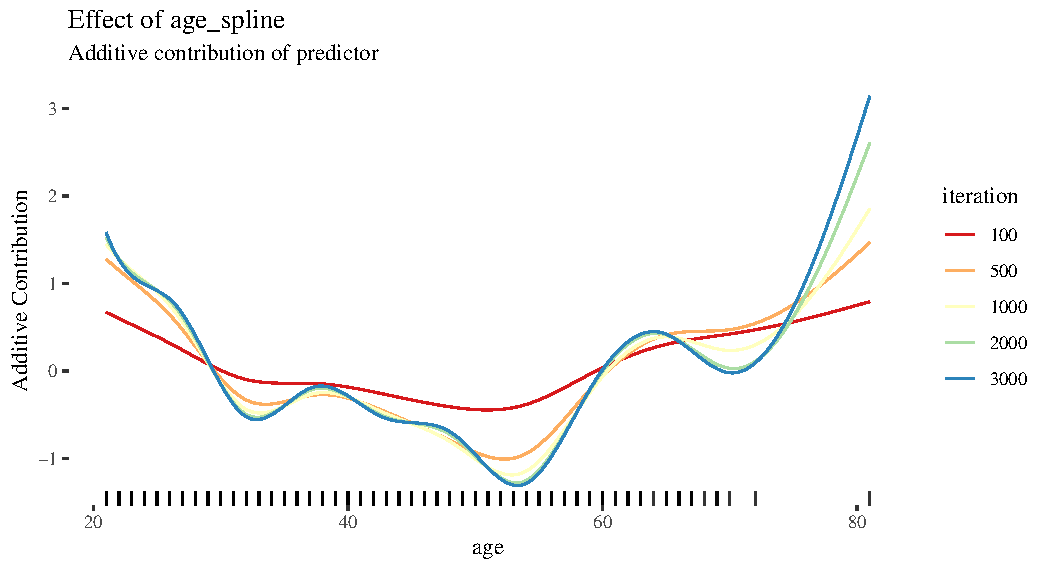
\includegraphics[width=11cm,height=6cm]{figure/unnamed-chunk-12-1} 

\end{knitrout}
\end{center}

\end{frame}

\begin{frame}[fragile]{Custom Loss: Definition}

As an example we want to define a custom loss corresponding to the Poisson distribution:

\begin{knitrout}
\definecolor{shadecolor}{rgb}{0.969, 0.969, 0.969}\color{fgcolor}\begin{kframe}
\begin{alltt}
\hlstd{lossPoisson} \hlkwb{=} \hlkwa{function} \hlstd{(}\hlkwc{truth}\hlstd{,} \hlkwc{response}\hlstd{) \{}
  \hlkwd{return} \hlstd{(}\hlopt{-}\hlkwd{log}\hlstd{(}\hlkwd{exp}\hlstd{(response)}\hlopt{^}\hlstd{truth} \hlopt{*} \hlkwd{exp}\hlstd{(}\hlopt{-}\hlkwd{exp}\hlstd{(response))} \hlopt{/} \hlkwd{gamma}\hlstd{(truth} \hlopt{+} \hlnum{1}\hlstd{)))}
\hlstd{\}}
\hlstd{gradPoisson} \hlkwb{=} \hlkwa{function} \hlstd{(}\hlkwc{truth}\hlstd{,} \hlkwc{response}\hlstd{) \{}
  \hlkwd{return} \hlstd{(}\hlkwd{exp}\hlstd{(response)} \hlopt{-} \hlstd{truth)}
\hlstd{\}}
\hlstd{constInitPoisson} \hlkwb{=} \hlkwa{function} \hlstd{(}\hlkwc{truth}\hlstd{) \{}
  \hlkwd{return} \hlstd{(}\hlkwd{log}\hlstd{(}\hlkwd{mean.default}\hlstd{(truth)))}
\hlstd{\}}
\hlcom{# Define custom loss:}
\hlstd{my.poisson.loss} \hlkwb{=} \hlstd{CustomLoss}\hlopt{$}\hlkwd{new}\hlstd{(lossPoisson, gradPoisson, constInitPoisson)}
\end{alltt}
\end{kframe}
\end{knitrout}

\end{frame}


\begin{frame}[fragile]{Custom Loss: Train Model}

\begin{knitrout}
\definecolor{shadecolor}{rgb}{0.969, 0.969, 0.969}\color{fgcolor}\begin{kframe}
\begin{alltt}
\hlkwd{data}\hlstd{(VonBort,} \hlkwc{package} \hlstd{=} \hlstr{"vcd"}\hlstd{)}

\hlcom{# Run compboost with custom loss:}
\hlstd{cboost} \hlkwb{=} \hlstd{Compboost}\hlopt{$}\hlkwd{new}\hlstd{(VonBort,} \hlstr{"deaths"}\hlstd{,} \hlkwc{loss} \hlstd{= my.poisson.loss)}
\hlstd{cboost}\hlopt{$}\hlkwd{addBaselearner}\hlstd{(}\hlstr{"year"}\hlstd{,} \hlstr{"spline"}\hlstd{, PSplineBlearner)}
\hlstd{cboost}\hlopt{$}\hlkwd{train}\hlstd{(}\hlnum{100}\hlstd{,} \hlkwc{trace} \hlstd{=} \hlnum{FALSE}\hlstd{)}

\hlcom{# Run mboost with pre-defined Poisson family:}
\hlstd{mod} \hlkwb{=} \hlkwd{mboost}\hlstd{(deaths} \hlopt{~} \hlkwd{bbs}\hlstd{(year,} \hlkwc{lambda} \hlstd{=} \hlnum{2}\hlstd{),} \hlkwc{data} \hlstd{= VonBort,} \hlkwc{family} \hlstd{=} \hlkwd{Poisson}\hlstd{(),}
  \hlkwc{control} \hlstd{=} \hlkwd{boost_control}\hlstd{(}\hlkwc{mstop} \hlstd{=} \hlnum{100}\hlstd{,} \hlkwc{nu} \hlstd{=} \hlnum{0.05}\hlstd{))}

\hlkwd{head}\hlstd{(}\hlkwd{data.frame}\hlstd{(}
  \hlkwc{compboost} \hlstd{= cboost}\hlopt{$}\hlkwd{coef}\hlstd{()[[}\hlstr{"year_spline"}\hlstd{]],}
  \hlkwc{mboost} \hlstd{=} \hlkwd{coef}\hlstd{(mod)[[}\hlstr{"bbs(year, lambda = 2)"}\hlstd{]]))}
\end{alltt}
\begin{verbatim}
##   compboost  mboost
## 1   -1.2233 -1.2233
## 2   -0.9133 -0.9133
## 3   -0.6078 -0.6078
## 4   -0.3389 -0.3389
## 5   -0.1809 -0.1809
## 6   -0.0788 -0.0788
\end{verbatim}
\end{kframe}
\end{knitrout}

\end{frame}

\section{Benchmark}


\begin{frame}[fragile]{Runtime Comparison With Mboost}

\begin{center}
\begin{knitrout}
\definecolor{shadecolor}{rgb}{0.969, 0.969, 0.969}\color{fgcolor}\begin{figure}
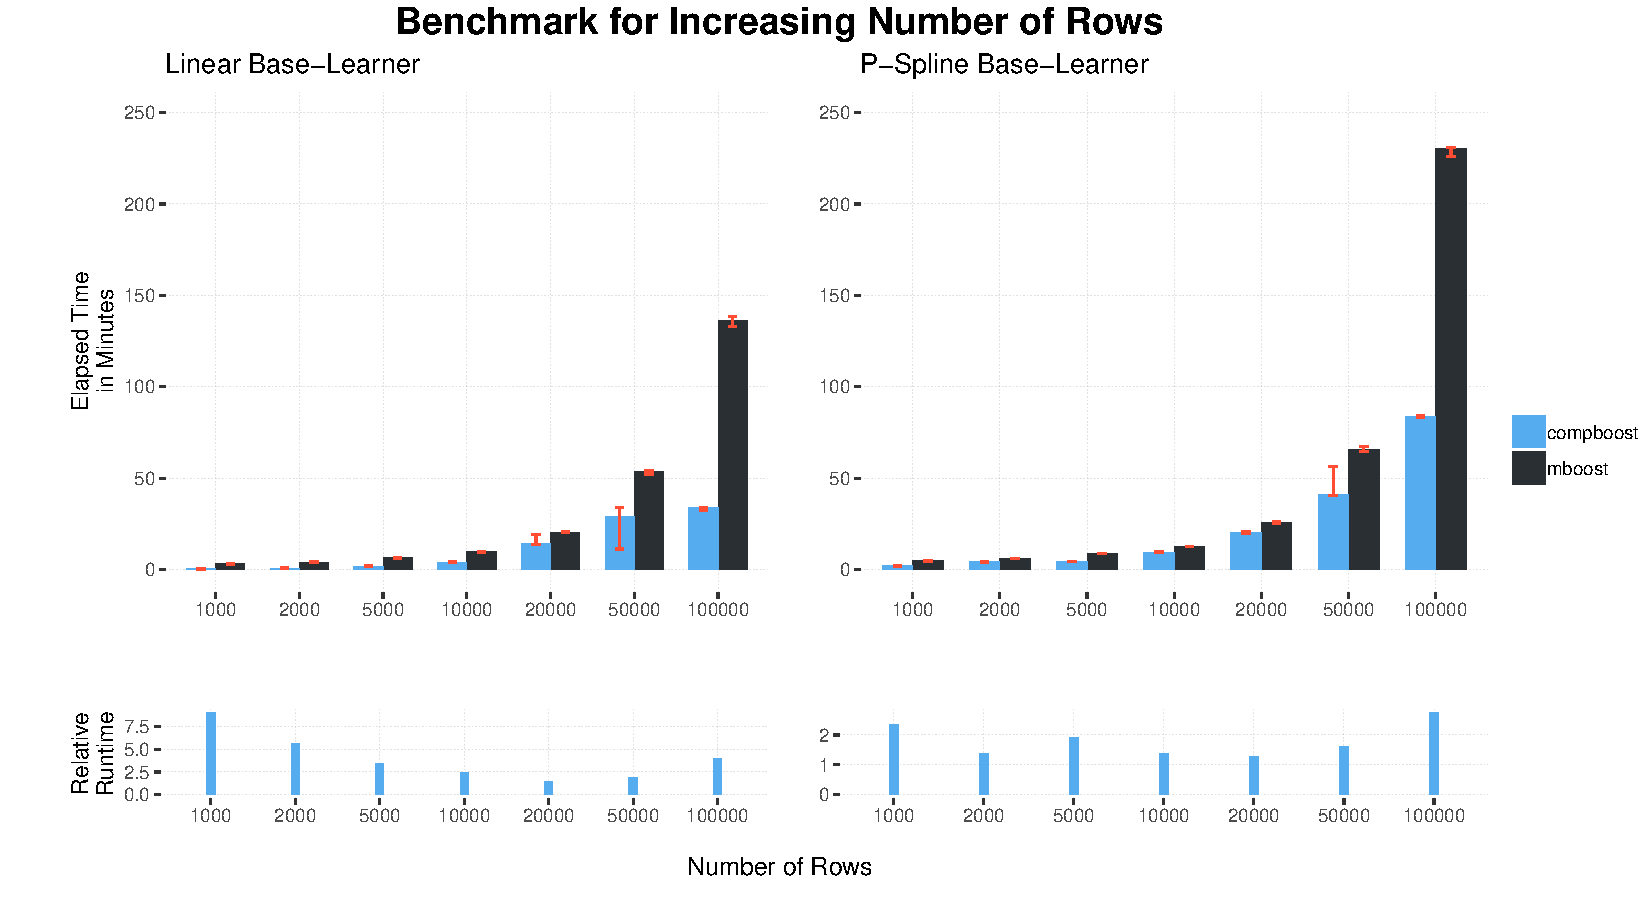
\includegraphics[width=11cm,height=6cm]{figure/unnamed-chunk-15-1} \caption[Runtime benchmark on simulated data with 2000 iterations and 1000 base-learner]{Runtime benchmark on simulated data with 2000 iterations and 1000 base-learner.}\label{fig:unnamed-chunk-15}
\end{figure}


\end{knitrout}
\end{center}

\end{frame}


\begin{frame}{Memory Comparison With Mboost}

\begin{center}
\begin{knitrout}
\definecolor{shadecolor}{rgb}{0.969, 0.969, 0.969}\color{fgcolor}\begin{figure}
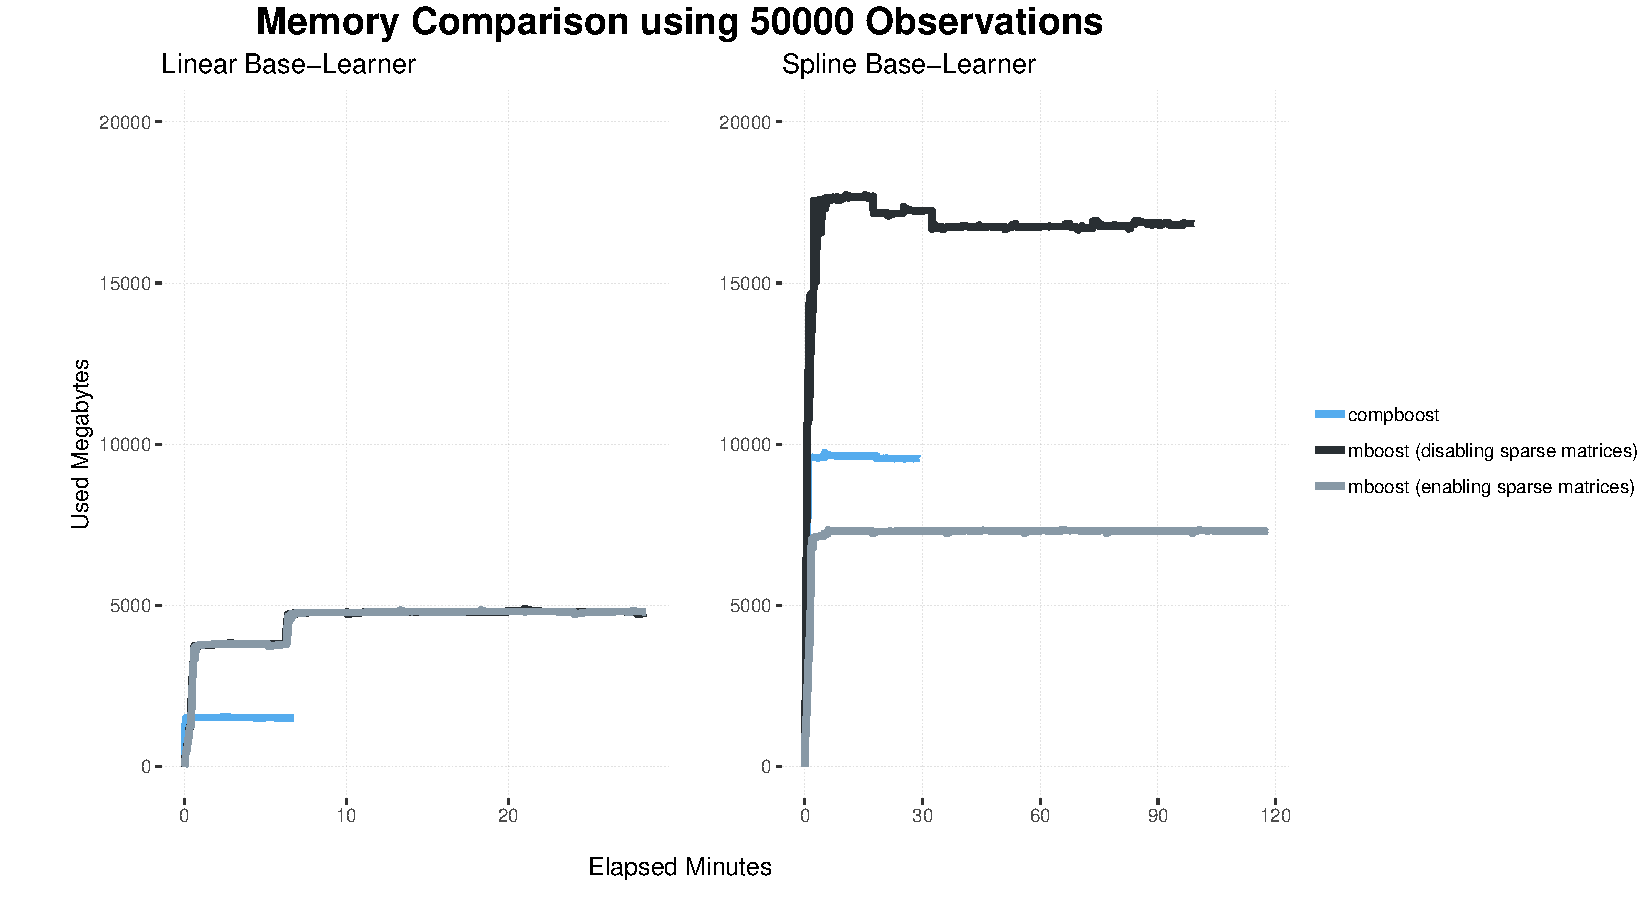
\includegraphics[width=11cm,height=6cm]{figure/unnamed-chunk-16-1} \caption[Memory benchmark on simulated data with 1000 iterations, 50000 observations, and 1000 base-learner]{Memory benchmark on simulated data with 1000 iterations, 50000 observations, and 1000 base-learner.}\label{fig:unnamed-chunk-16}
\end{figure}


\end{knitrout}
\end{center}

\end{frame}

\section{Next Steps}


\begin{frame}{Next Steps}

\begin{itemize}

  \item
    Implementing more base-learner and loss functions.
    
  \item
    Adding support for multiclass classification.
    
  \item
    Running the algorithm in parallel.
    
  \item 
    Using sparse matrices to store, e.g., spline data matrices.
    
  \item 
    Releasing the package on \textit{CRAN}.

\end{itemize}

\end{frame}

\begin{frame}{Where to Find}

\begin{itemize}

  \item
    Developed on \emph{GitHub}:
    \begin{center}
      \url{www.github.com/schalkdaniel/compboost}
    \end{center}

  \item 
    Additional resources on the project page:
    \begin{center}
    	\url{www.compboost.org}
    \end{center}

  \item 
  	Bug reports via the \href{https://github.com/schalkdaniel/compboost/issues}{issue tracker}.

\end{itemize}
\vspace{0.4cm}
\begin{center}
\textbf{Contributions are highly welcome!}
\end{center}
\end{frame}

\appendix

% \begin{frame}[plain, standout]
%   Questions?
% \end{frame}

\begin{frame}[plain]{References}
\vphantom{\cite{sanderson2016armadillo}}
\begingroup
  \renewcommand{\section}[2]{}
  \scriptsize
  \bibliographystyle{apalike}
  \bibliography{bibliography}
\endgroup
\end{frame}

\end{document}
